\documentclass{article}

\usepackage[utf8]{inputenc}
\usepackage[T1]{fontenc}
\usepackage[greek,english]{babel}
\usepackage{alphabeta}
\usepackage{amsmath}
\usepackage{amssymb}
\usepackage{graphicx}
\usepackage{subcaption}
\usepackage{epstopdf}
\usepackage[margin=1in, paperwidth=7.5in,paperheight=10.5in]{geometry}
\usepackage{hyperref}
\usepackage{paracol}

\newcommand\course{TΗΛ411}
\newcommand\courseName{Ψηφιακή Επεξεργασία Εικόνας}
\newcommand\semester{Χειμερινό 2021}
\newcommand\assignmentNumber{Assignment 6}
\newcommand\studentName{Μαυρογιώργης Δημήτρης}                           
\newcommand\studentNumber{2016030016}

\title{\underline{\textbf{\assignmentNumber}}} 
\author{\textsc{\textbf{Όνομα:}}  \studentName\\
		\textsc{\textbf{ΑΜ:}}  \studentNumber\\
		\course \ - \courseName\\ 
		\textsc{Πολυτεχνείο Κρήτης}
}
\date{\today}
\begin{document}
	\maketitle

\section*{Introduction}
	Ο σκοπός της 6ης εργαστηριακής άσκησης είναι να εντοπίσουμε σε μία φωτογραφία που λήφθηκε από δορυφόρο μια κατοικημένη περιοχή. Ειδικότερα, το πρόβλημα αυτό έχει να κάνει με τον εντοπισμό διαφορετικών υφών, καθώς μία κατοικημένη περιοχή έχει διαφορετική υφή από μια αγροτική περιοχή.
	
\section*{Implementation-Results}
	Στο πρώτο σκέλος της άσκησης, έπρεπε να κάνουμε binary την εικόνα που μας δώθηκε, δοκιμάζοντας διαφορετικές τιμές του threshhold στο διάστημα [0,1]. Για το βήμα αυτό χρησιμοποιήθηκε η im2bw συνάρτηση της matlab, στην οποία δώθηκαν ως όρισμα το map της εικόνας και το threshhold. Μετά από δοκιμές για τις διάφορες τιμές threshhold, βρέθηκε ότι η βέλτιστη τιμή είναι 0.5. Για τις υπολοιπες τιμές η εικόνα ήταν όλη μαύρη ή άσπρη ή δεν απεικονιζόταν με αρκετή λεπτομέρεια η κατοικημένη περιοχή.
	 
	\begin{figure}[h!]
		\centering
		\begin{subfigure}[t]{0.5\textwidth}
			\centering
			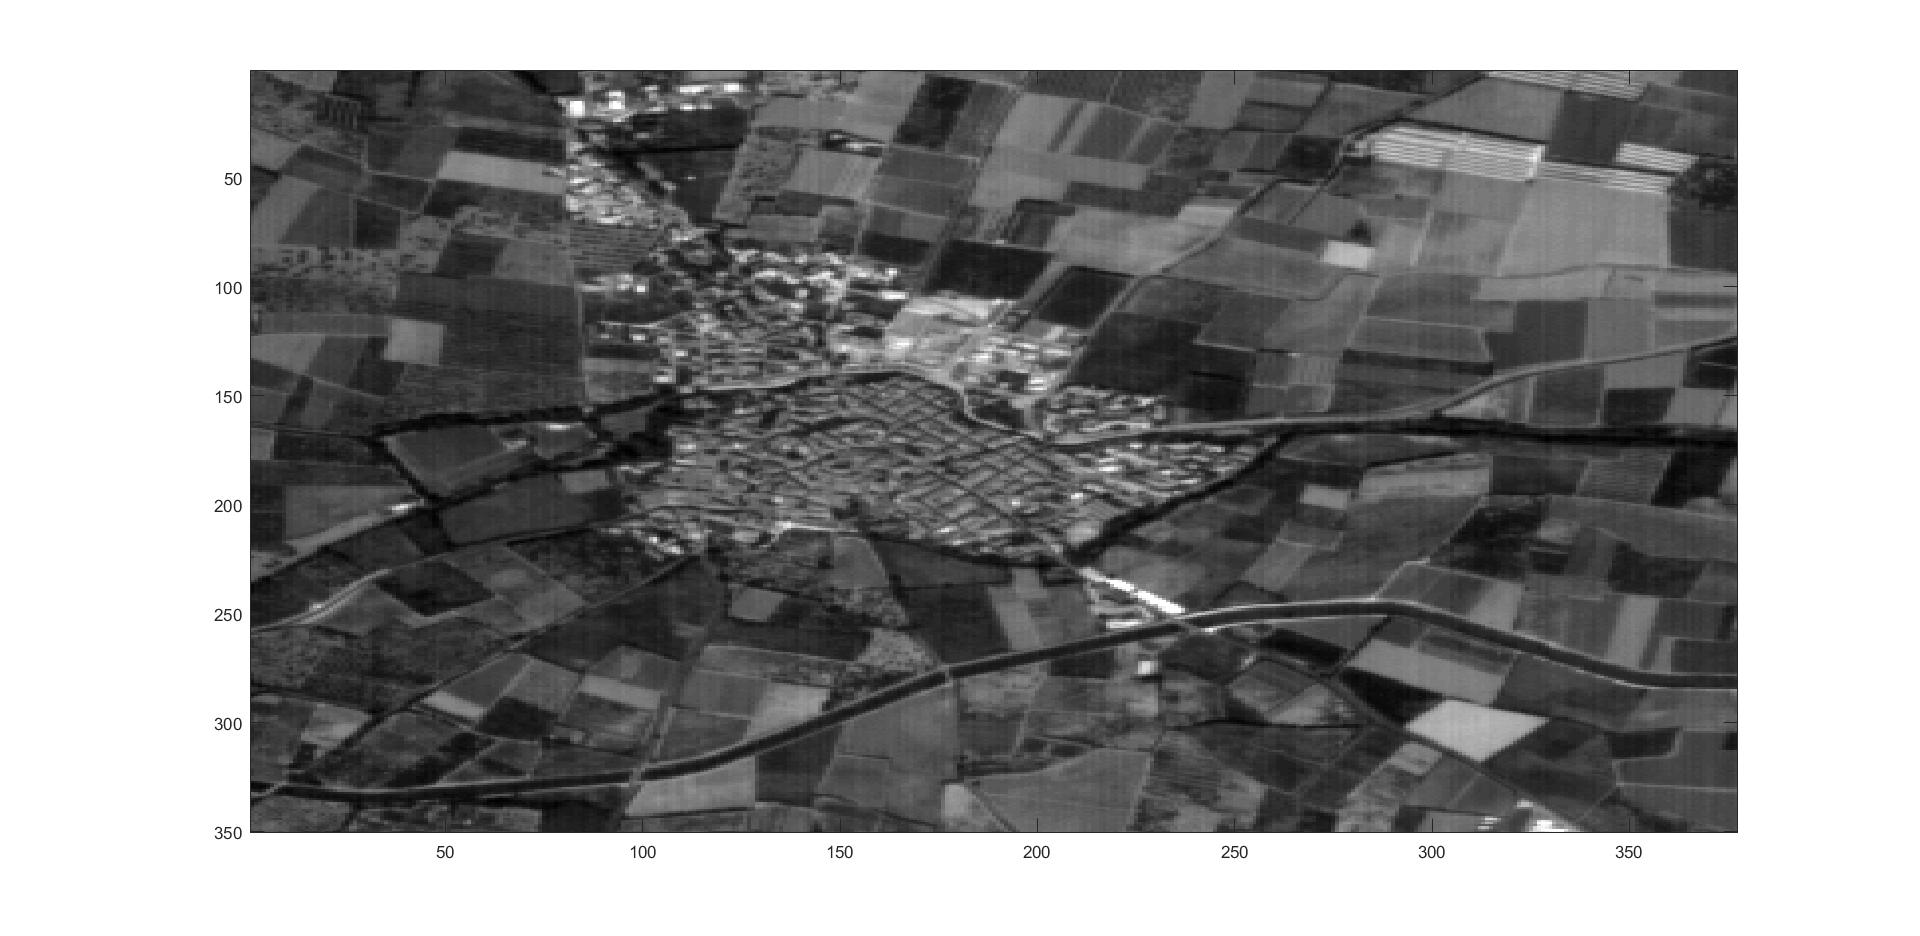
\includegraphics[height=\linewidth, width=\linewidth]{./output_images/village.jpg}
		\end{subfigure}%
		~
		\begin{subfigure}[t]{0.5\textwidth}
			\centering
			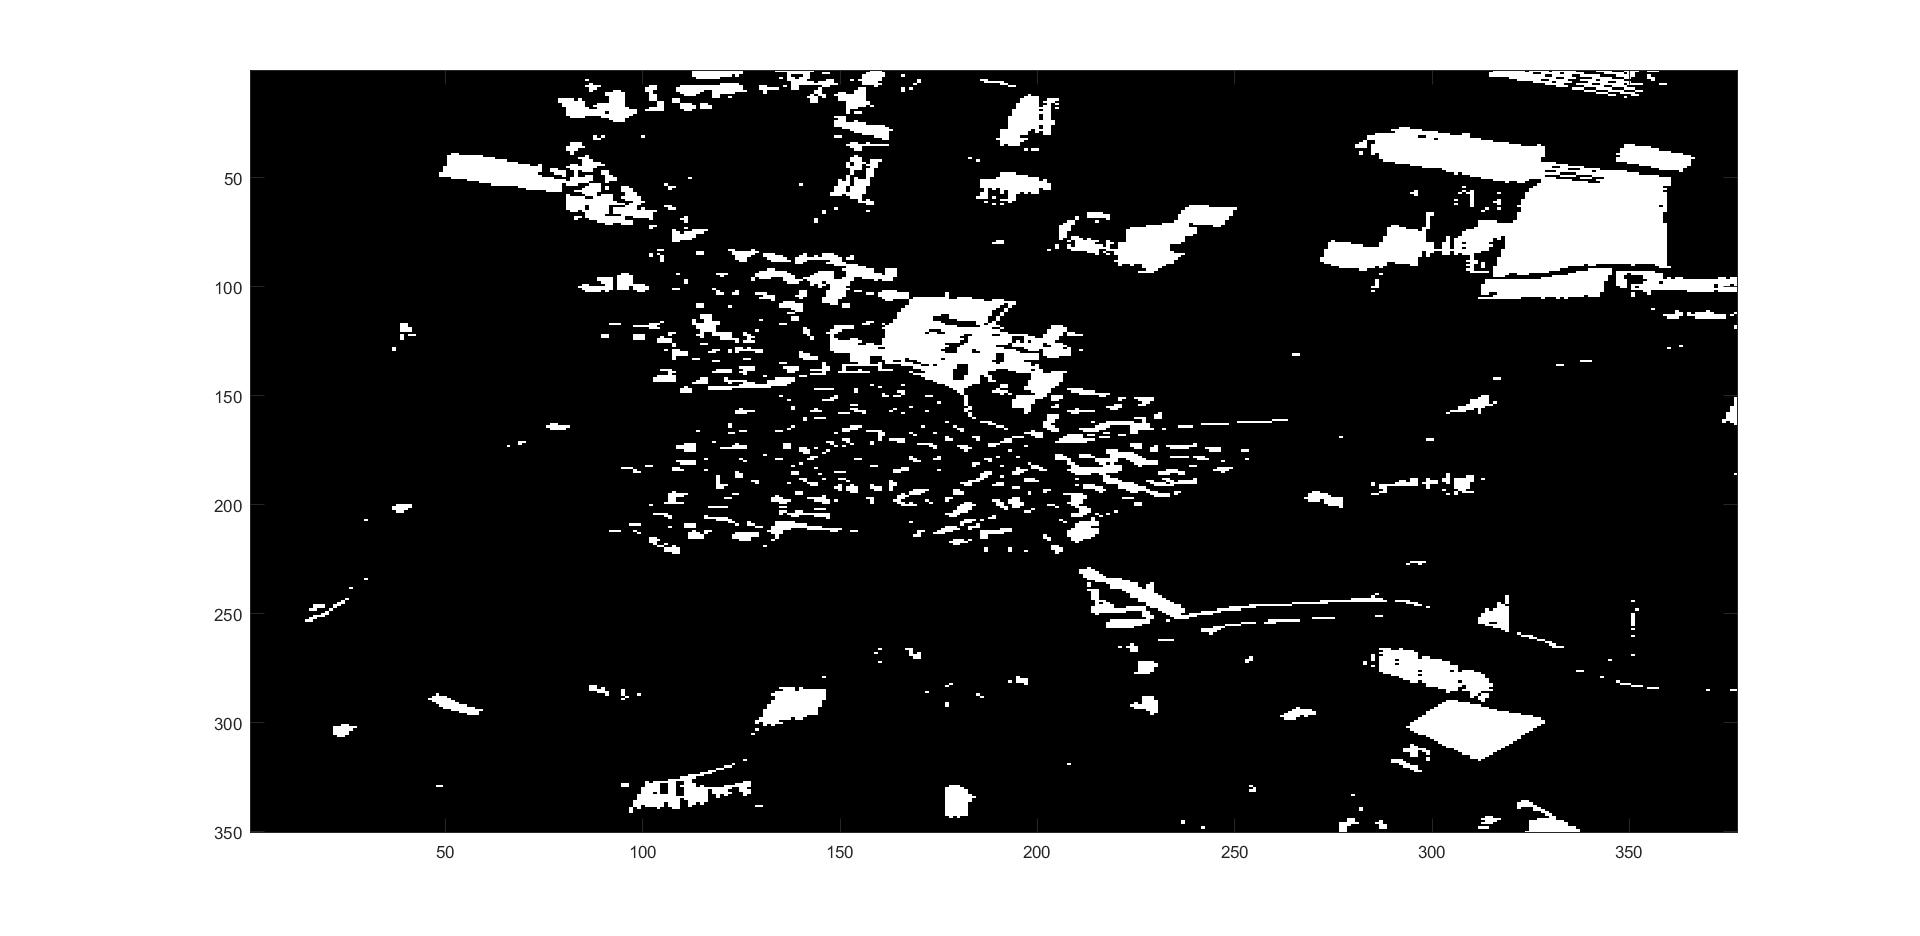
\includegraphics[height=\linewidth, width=\linewidth]{./output_images/lab6_step1.jpg}
		\end{subfigure}	
		\caption{Application of 3x3, 5x5 and 9x9 Median filter to two different noisy images}
	\end{figure}

	\pagebreak
	\noindent                                                                                   
	Στο δεύτερο σκέλος της άσκησης, μας δώθηκε μια συνάρτηση "UrbanDetec.m", η οποία με την μέθοδο window sliding επεξεργάζεται στατιστικά την εικόνα χρησιμοποιώντας την μέθοδο της διακύμανσης, ώστε να εντοπίσει την κατοικημένη περιοχή. Και σε αυτό το σκέλος έπρεπε να δοκιμάσουμε διαφορετικές τιμές για το window, το οποίο παίρνει τιμές 3, 5, 7 κλπ, και για το threshhold και να απεικονίσουμε το βέλτιστο αποτέλεσμα. Έπειτα από δοκιμές βρέθηκε ότι οι βέλτιστες τιμές για window και threshhold είναι 3 και 0.1 αντίστοιχα.

	\begin{figure}[h!]
		\centering
		\begin{subfigure}[t]{0.5\textwidth}
			\centering
			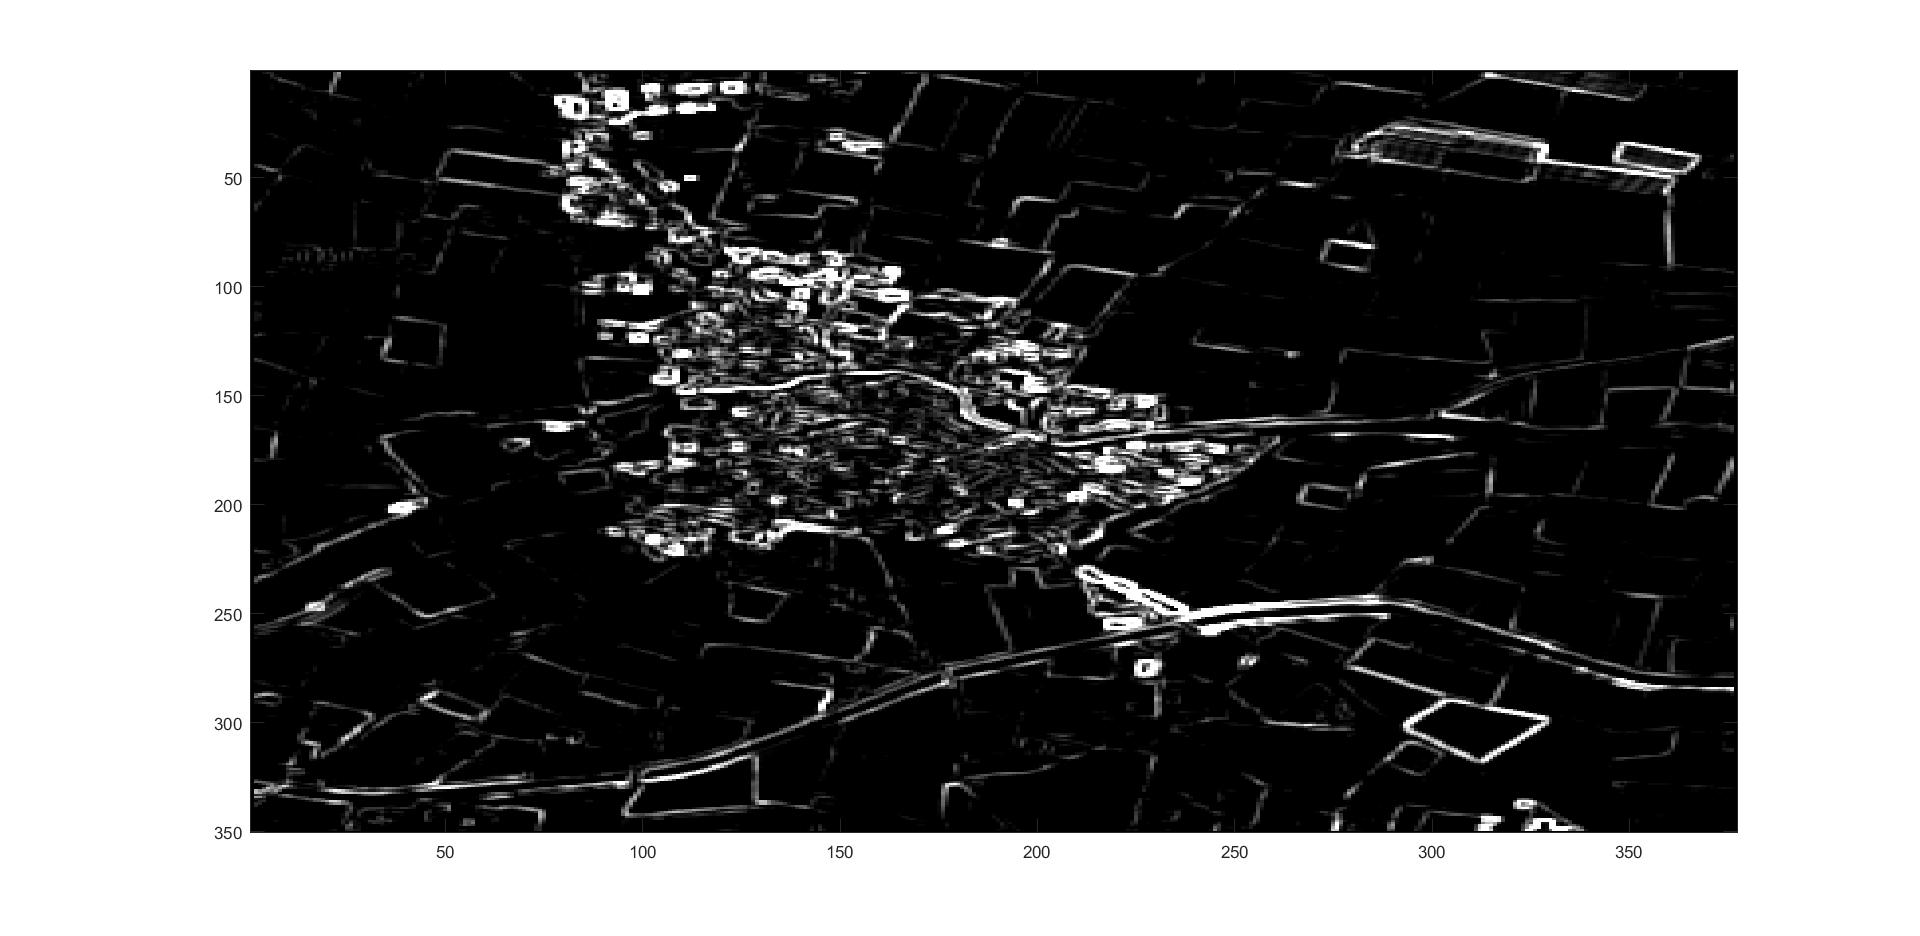
\includegraphics[height=\linewidth, width=\linewidth]{./output_images/lab6_step2a.jpg}
		\end{subfigure}%
		~
		\begin{subfigure}[t]{0.5\textwidth}
			\centering
			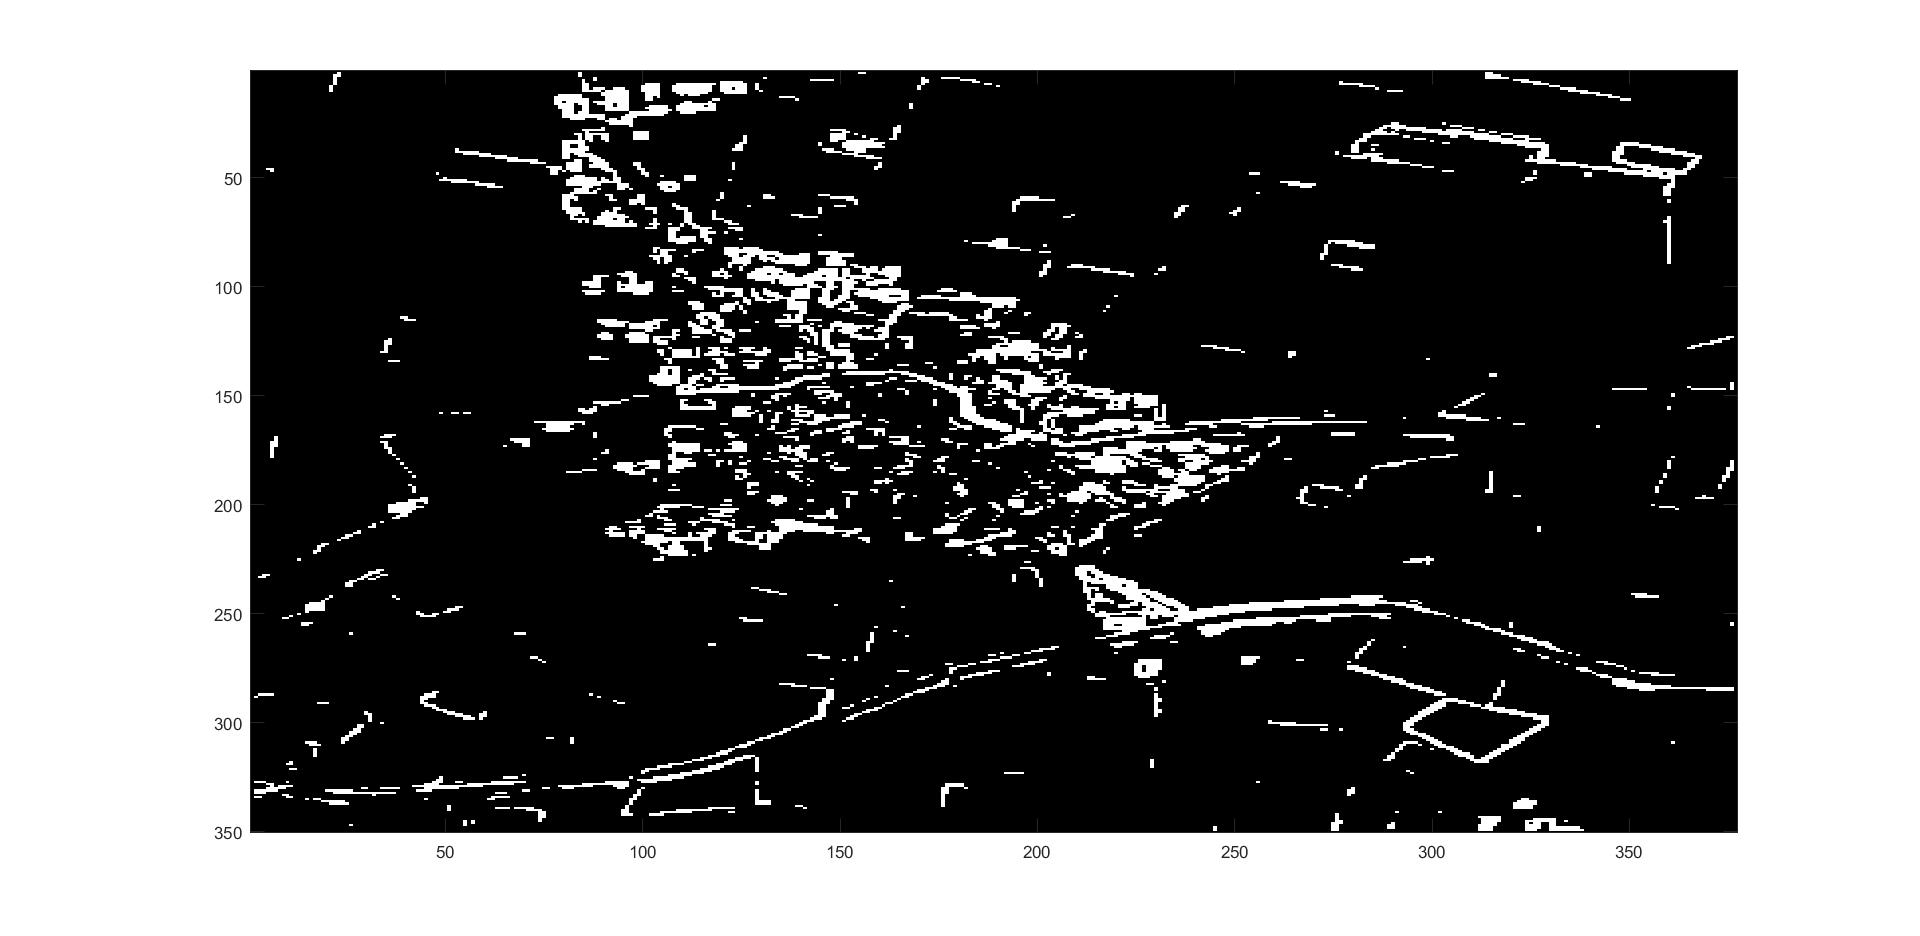
\includegraphics[height=\linewidth, width=\linewidth]{./output_images/lab6_step2b.jpg}
		\end{subfigure}	
	\end{figure}
	
	\noindent
	Aυτό που παρατηρούμε συγκρίνοντας το βήμα 1 με το βήμα 2 της άσκησης είναι ότι στη δεύτερη περίπτωση τα αποτελέσματα είναι καλύτερα, δηλαδή με τη στατιστική επεξεργασία της εικόνας μπορούμε να απεικονίσουμε με μεγαλύτερη λεπτομέρεια την κατοικημέση περιοχή. Επίσης, παρατηρήθηκε ότι για μέγεθος παραθύρου μεγαλύτερο του 3 τα αποτελέσματα ήταν χειρότερα. Τέλος, για μεγεθος παραθύρου 3 και διαφορετικές τιμές threshhold μεγαλύτερες του 0.1, παρατηρήθηκε ότι η μέθοδος του βήματος 2 δεν απεικόνιζε με μεγάλη λεπτομέρεια την κατοικημένη περιοχή και χανόταν πληροφορία.\\
	
	\noindent
	Στο τελευταίο κομμάτι της άσκησης, ο στόχος είναι να εντοπίσουμε το χωριό χρησιμοποιώντας τεχνικές μορφολογικής επεξεργασίας μιας εικόνας. Πιο συγκεκριμένα, μας δώθηκαν τα βήματα ενός αλγορίθμου που έπρεπε να ακολουθήσουμε για να εντοπίσουμε την κατοικημένη περιοχή.\\
	
	\noindent
	Στο 1ο βήμα ζητήθηκε να εφαρμόσουμε το Top-Hat και Bottom-Hat φίλτρο στην αρχική εικόνα. Για το λόγο αυτό χρησιμοποιήθηκαν οι συναρτήσεις imerode και imdilate. Για τον TH υπολογισμό έγινε αφαίρεση από την αρχική εικόνα το αποτέλεσμα που προέκυψε από την imerode ακολουθούμενη από imdilate. Αντιστροφα, για το BH, αφού έγινε πρώτα imdilate ακολουθούμενο από imerode, αφαιρέθηκε η αρχική εικόνα. Για τον υπολογισμο των TH και BH χρησιμοποιήθηκε ως αντικείμενο ένα square 3x3. 	
	
	\pagebreak
	\begin{figure}[h!]
		\centering
		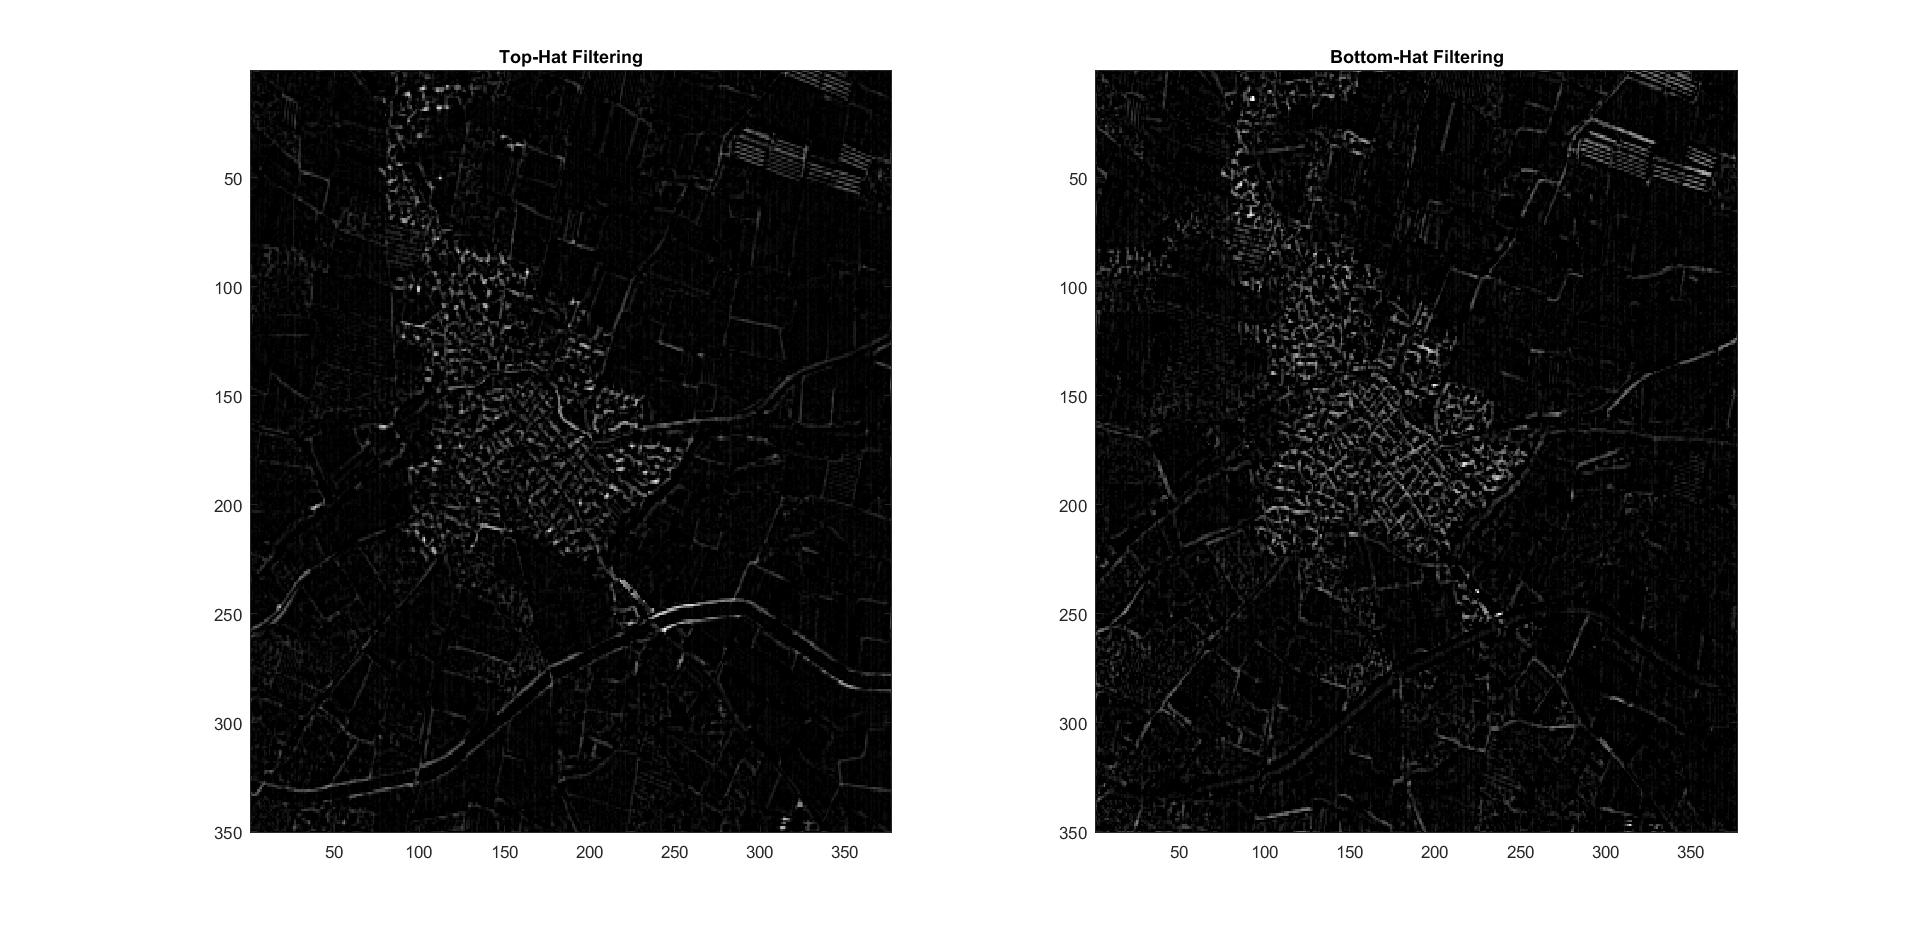
\includegraphics[ width=\linewidth]{./output_images/lab6_step3a.jpg}
	\end{figure}
	
	\noindent
	Στο 2ο και 3ο βήμα έπρεπε να κανονικοποιήσουμε την εικόνα και να χρησιμοποιήσουμε τη μέθοδο Otsu για τον υπολογισμό ενός βέλτιστου κατωφλιού χρησιμοποιώντας τη συνάρτηση graythresh. Στη συνέχεια, στο βήμα 4 του αλγορίθμου χρησιμοποιήθηκε η συνάρτηση im2bw για να γίνουν binary οι εικόνες TH και BH, στην οποία χρησιμοποιήθηκε το κατώφλι από τη μέθοδο Otsu.
	
	\begin{figure}[h!]
		\centering
		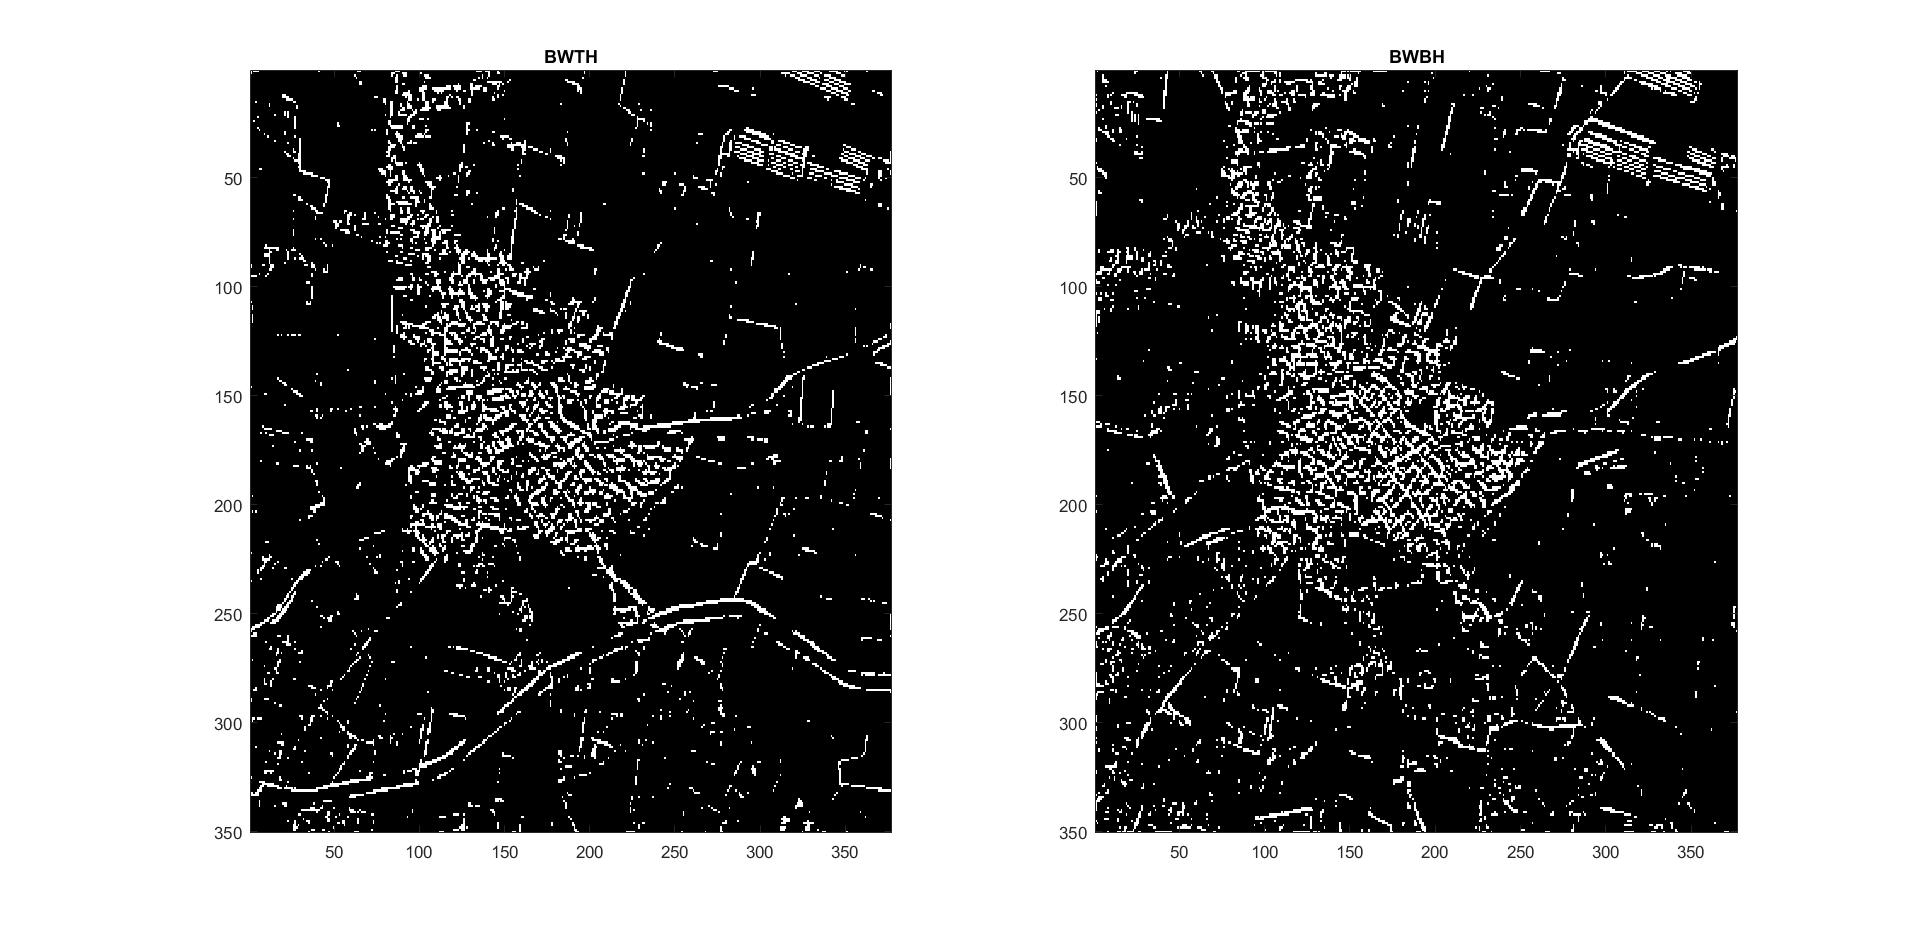
\includegraphics[ width=\linewidth]{./output_images/lab6_step3b.jpg}
	\end{figure}
	
	\pagebreak
	\noindent
	Στο βήμα 5, χρησιμοποιώντας τη συνάρτηση imopen έγινε το άνοιγμα της binary εικόνα TH, δηλαδή απομακρύνθηκαν από την εικόνα μικρά αντικείμενα, διατηρώντας όμως το σχήμα. Για τον υπολογισμο του βήματος 5 χρησιμοποιήθηκε ως αντικείμενο ένα square 2x2. Στο βήμα 6, χρησιμοποιώντας τις συναρτήσεις imclose και imopen αντίστοιχα, έγινε το κλείσιμο της binary εικόνας BH για το γέμισμα οπών και έπειτα ακολουθήθηκε από το άνοιγμα για να απομακρυνθούν πάλι μικρά αντικείμενα. Για τον υπολογισμο του βήματος 6 χρησιμοποιήθηκε ως αντικείμενο ένα diamond διάστασης 3x3, καθώς είχε καλύτερα αποτελέσματα από το square. 
	
	\begin{figure}[h!]
		\centering
		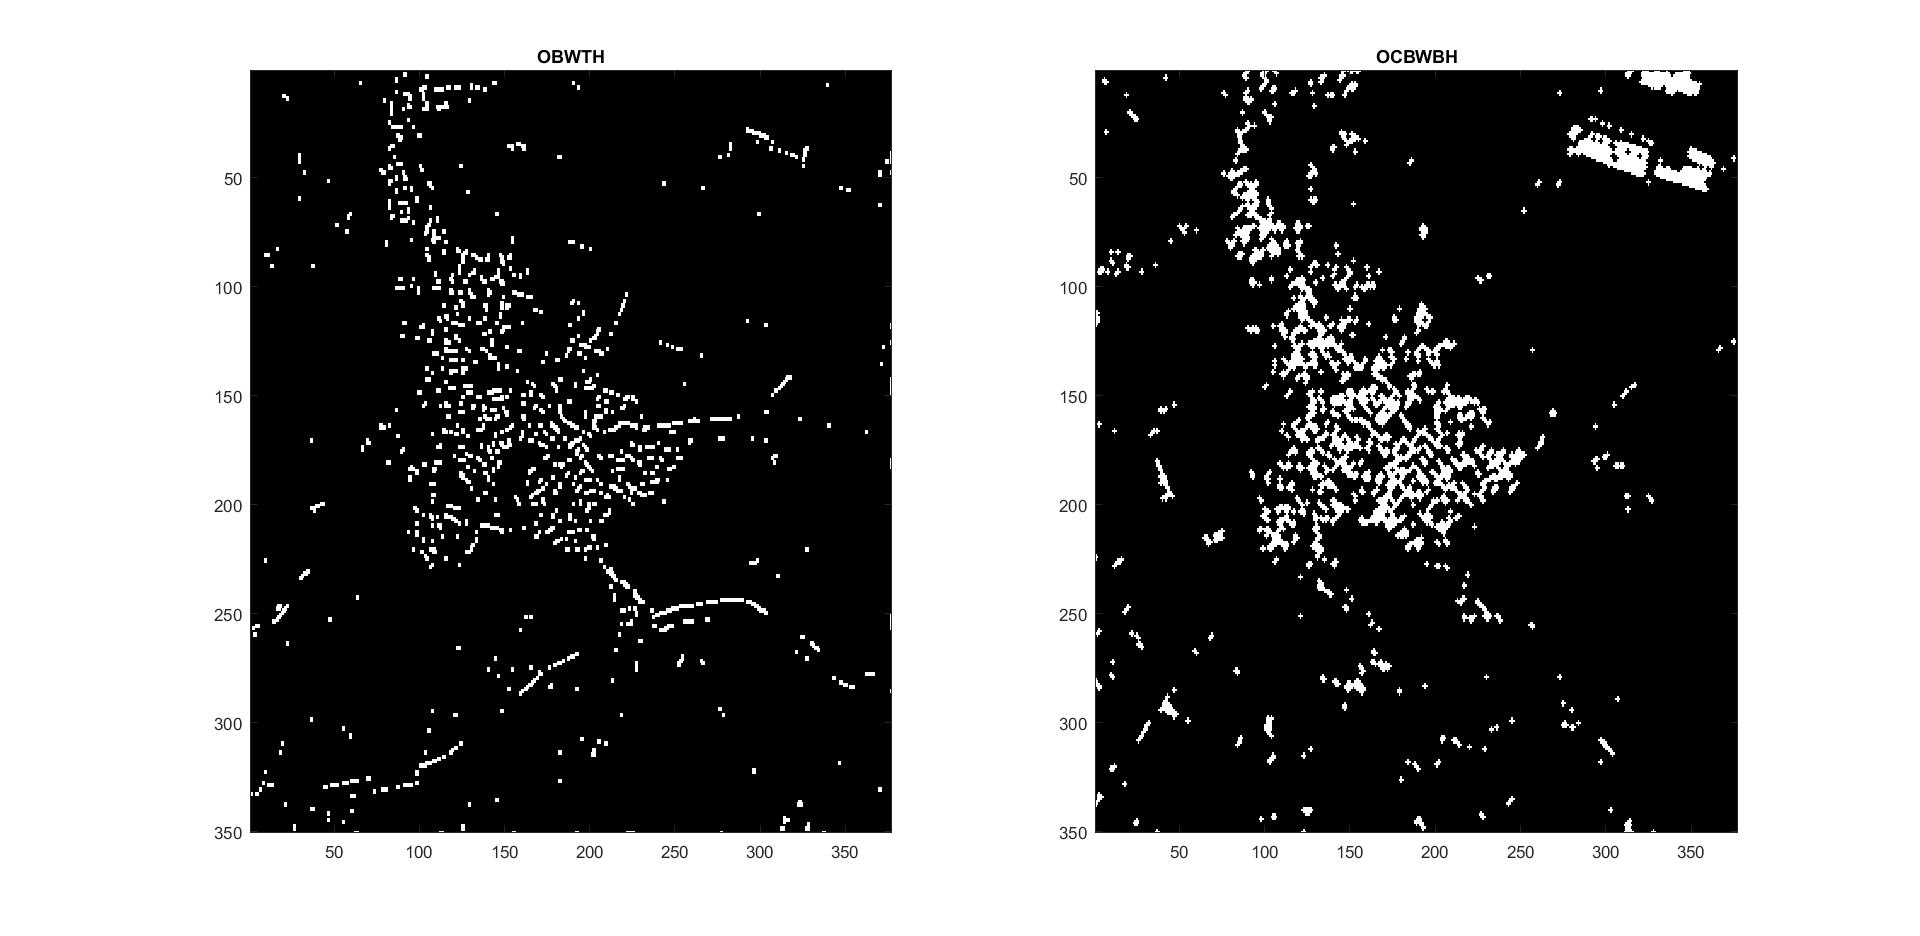
\includegraphics[ width=\linewidth]{./output_images/lab6_step3c.jpg}
	\end{figure}
	
	\noindent
	Tέλος, χρησιμοποιήθηκε η imfuse συνάρτηση με παράμετρο 'diff' για να προκύψει το τελικό αποτέλεσμα, δηλαδή ο εντοπιστμός της κατοικημένης περιοχής.
	
	\begin{figure}[h!]
		\centering
		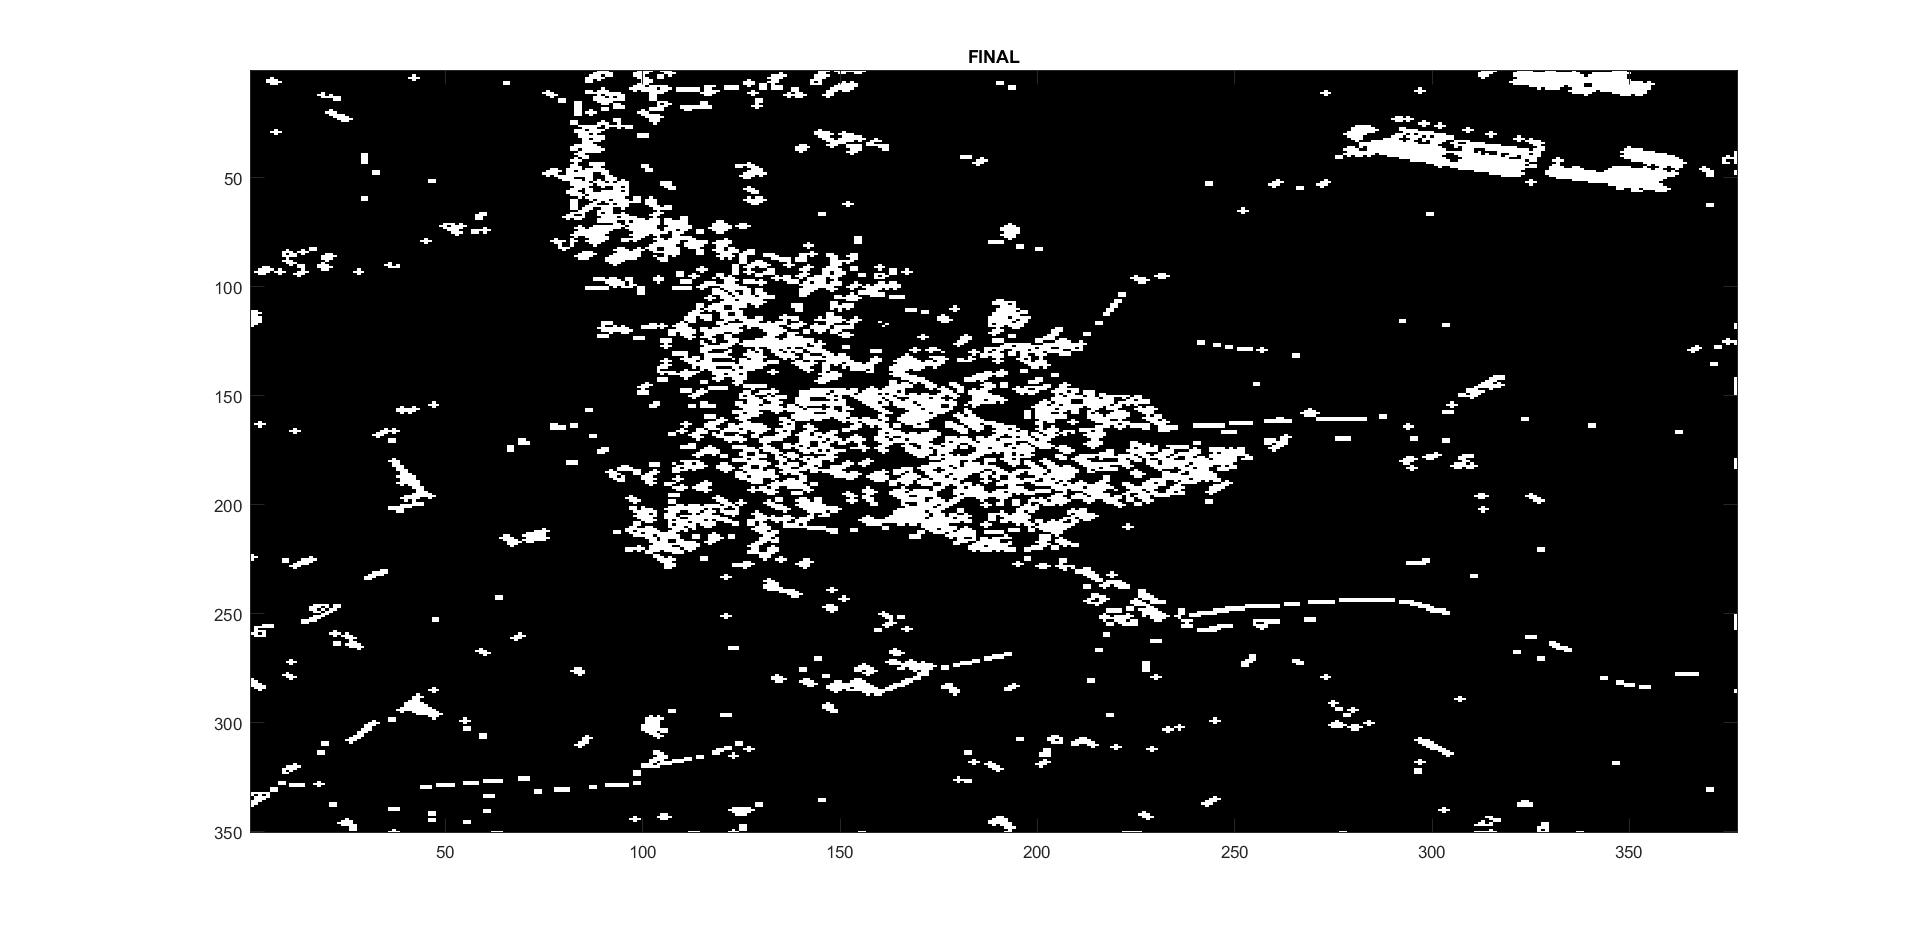
\includegraphics[ width=\linewidth]{./output_images/lab6_step3d.jpg}
	\end{figure}
	
	\noindent
	Γενικά, μετά από όλη την παραπάνω διαδικασία βλέπουμε ότι καταλήγουμε σε μια καλή απεικόνιση της κατοικημένης περιοχής. Το τελικό αποτέλεσμα εξαρτάται και από τα αντικείμενα που χρησιμοποιούμε σε κάθε βήμα, καθώς και από το βέλτιστο κατώφλι που προέκυψε από τη μέθοδο Otsu και χρησιμοποιούμε, για να κάνουμε binary τις TH και BH εικόνες.
\end{document}
